\documentclass[preprint]{elsarticle}
\usepackage{amssymb}
\usepackage{color}
\usepackage{pgf,pgfarrows,pgfnodes,pgfautomata,pgfheaps,pgfshade}
\usepackage{tikz}
\usetikzlibrary{arrows,automata,positioning}
\usetikzlibrary{arrows,decorations.pathmorphing,backgrounds,positioning,fit,petri}
\usepackage{amsmath}

\begin{document}

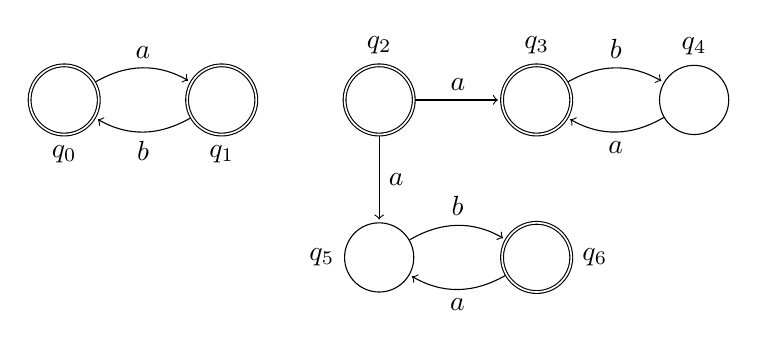
\begin{tikzpicture}[shorten >=1pt,node distance=2cm,on grid,auto]
 %primo-no
    
       \node[accepting,state,label={below:$q_0$}]            (q0)               {};
      \node[accepting,state,label={below:$q_1$}] (q1) [right of=q0] {};

      \path[->] (q0) edge   [bend left]     node {$a$} (q1)
                (q1) edge  [bend left] node {$b$}        (q0);
%secondo
       \node[accepting,state,label={above:$q_2$}] (q2)   [right of=q1]            {};
      \node[accepting,state, label={above:$q_3$}] (q3) [right of=q2] {};
      \node[state,label={above:$q_4$}]           (q4) [right of=q3] {};
      \node[state,label={left:$q_5$}]           (q5) [below of=q2] {};
        \node[accepting,state,label={right:$q_6$}]           (q6) [right of=q5] {};

      \path[->] (q2) edge node {$a$} (q3)
                    (q2) edge node {$a$} (q5)
                (q3) edge [bend left] node {$b$} (q4)
                  (q4)   edge  [bend left]   node {$a$} (q3)
                (q5) edge [bend left] node {$b$} (q6)
                (q6) edge [bend left] node {$a$} (q5);

    \end{tikzpicture}

\end{document}